\chapter{Results and Discussion}
The results presented here concern the effective three-body potential curves $U_{\nu}$. Signatures of the Efimov effect can be revealed in the structure of these adiabatic hyperspherical potentials; with the Efimov channel corresponding to the one emergent attractive potential converging to \eqref{eq:efimov_channel} in the region $r_0 \ll \rho \ll
\abs{a}$.

The adiabatic potential curves were obtained by numerically solving  \eqref{adiabatic} using the method described in \cref{chapter:5}. The setup described in this work was used to accurately reproduced the results presented by Blume in \cite{Blume2002}, which we show in \cref{fig:res_2}. The adiabatic potential curves were here numerically calculated with a potential strong enough to support two $s$-wave bound states and the potential depth $d$ was tuned to yeild a scattering length of $a=228$ a.u.. The adiabatic potential curves $U_{\nu}$ with $\nu = 0-7$ are plotted as functions of the hyperradius $\rho$. In this figure we can see that the two lowest potential curves $\nu = 0$ and $\nu = 1$ are converging to the two-body $s$-wave binding energies, which represents channels with one two-body bound  state plus a free particle. Here the channel index $\nu=1$ corresponds to the Efimov channel. The higher lying channels $\nu>1$ are continuum channels and the channel index $\nu=0$ represents a deeply bound state.

\begin{figure}
	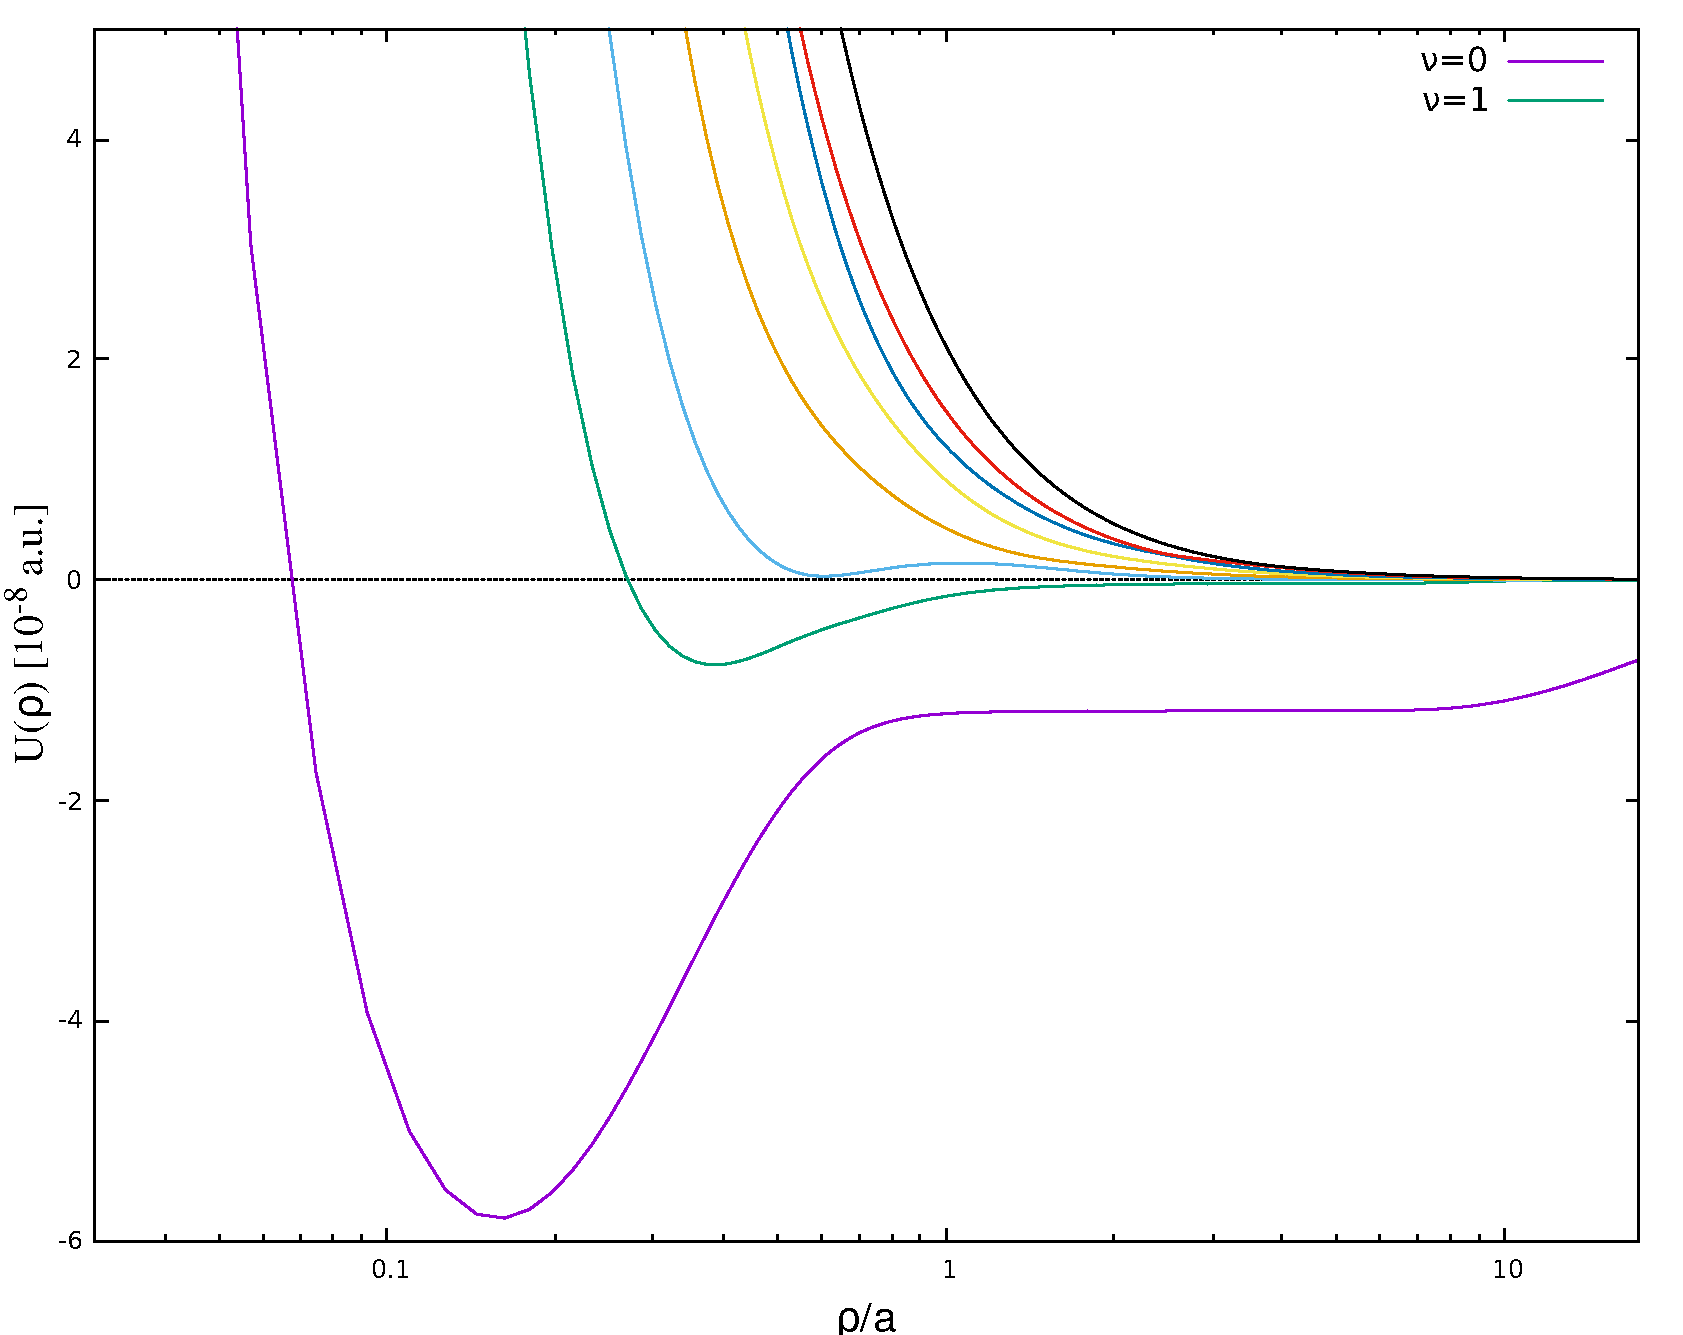
\includegraphics[width=\linewidth]{adiabatic.pdf}
	\caption{The adiabatic potential curves $U_{\nu}$ for $\nu=0-7$ are plotted as functions of the hyperradius $\rho$ for $a=228$ a.u. The index labelled $\nu=1$ correspond to the Efimov channel.}
	\label{fig:res_2}
\end{figure}

The results presented in \cref{fig:res_3,fig:res_4,fig:res_5,fig:res_6} were, in the cases where $a<0$, obtained by using values of $d$ which approached pole $\mathrm{I}$ from the right. For these values of $d$ the potential is too weak to support a two-body bound state. Similarly, for the results obtained for $a>0$ we used values of $d$ which approached pole $\mathrm{I}$ from the left, thus supporting a single two-body bound state. 

If \eqref{eq:efimov_channel} holds we expect the potential curves to converge towards \eqref{eq:efimov_channel} for $\abs{a} \rightarrow \infty$. This behaviour should be evident if the potentials are multiplied by $2 \mu \rho^2$ and plotted as 

\begin{equation}\label{eq:lambda}
2 \mu \rho^2 U_{\nu}(\rho) + \frac{1}{4},
\end{equation}
since these curves should approach the universal value $-s_0^2 (\simeq -1.0125$ for $J=0^+$ states).

In \cref{fig:res_3} the potential curves asymptotically associated with the lowest continuum channel for $a<0$ are plotted as functions of the hyperradius $\rho$ for four different values of $a$. As $\rho \rightarrow \infty$, the curves approach the eigenvalues of the kinetic energy, which correspond to $\lambda(\lambda + 4) + 4$ with $\lambda = 0$. In the intermediate region, the two effective potentials for the largest $\abs{a}$ seem to converge to $-s_0^2$ (the straight dashed line in \cref{fig:res_3}). 

\begin{figure}
	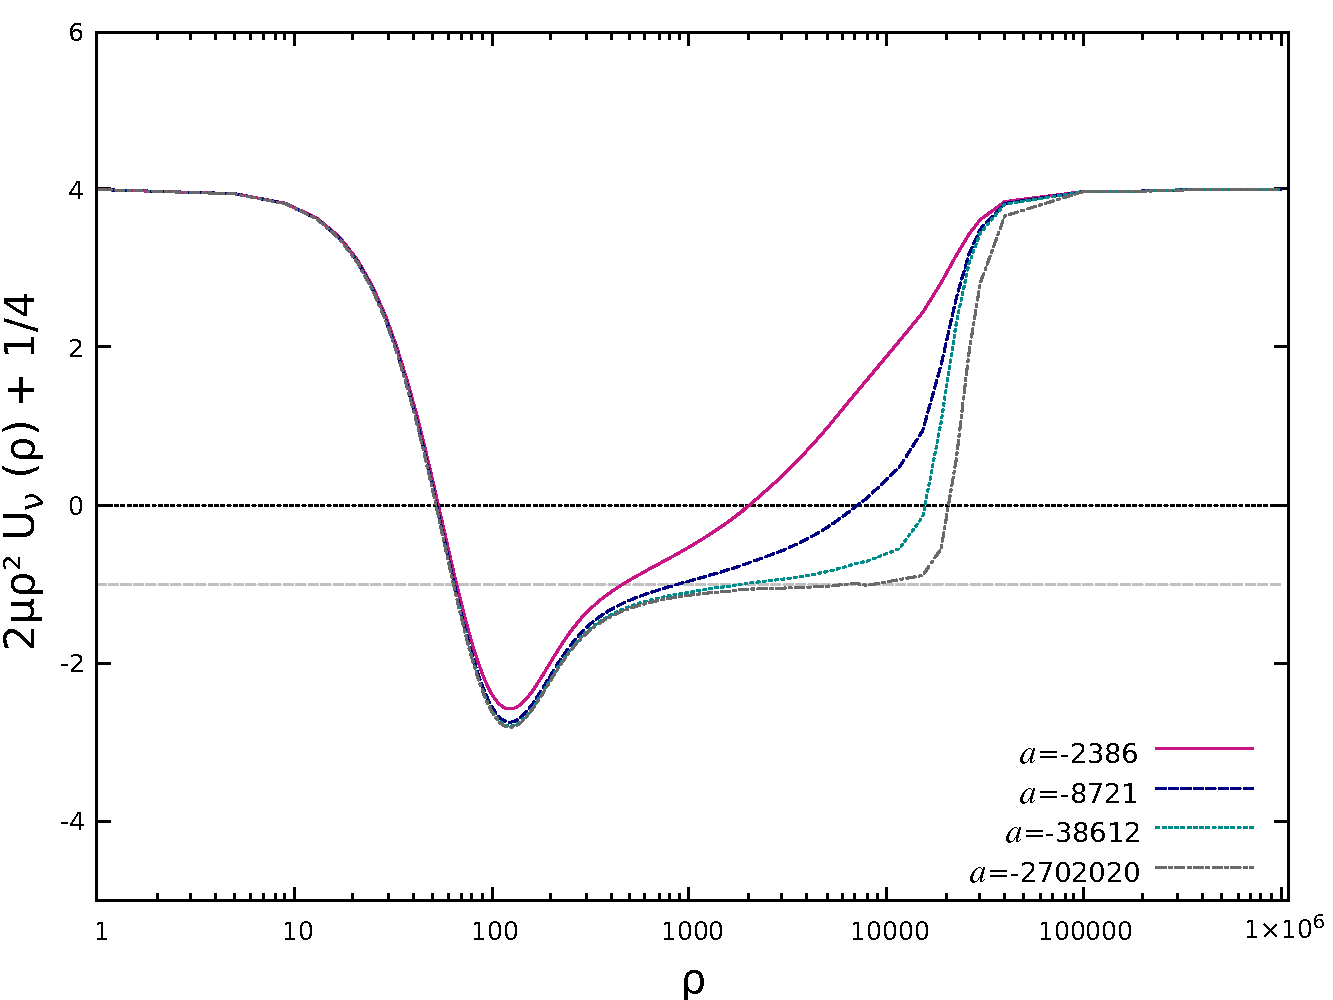
\includegraphics[width=\linewidth]{plotneg_dashed.pdf}
	\caption{Three-body effective potentials for $a<0$. The horizontal dashed line is the value $-s_0^2$, which the Efimov potential takes on for $\rho\gg r_0$.}
	\label{fig:res_3}
\end{figure}
Convergence of the curve for $a \rightarrow -\infty$ was checked by computing this potential curve for two different number of mesh points $N_{\theta}=N_{\phi}=80$ and $100$, see \cref{fig:res_4}. The potential curve obtained with a larger number of mesh points can be seen to converge to $-s_0^2$ in the intermediate region at hyperradii up to approximately $\rho=8000$ a.u.. However, we were not able to get convergence for $\rho>1 \times 10^4$ a.u. 

\begin{figure}
	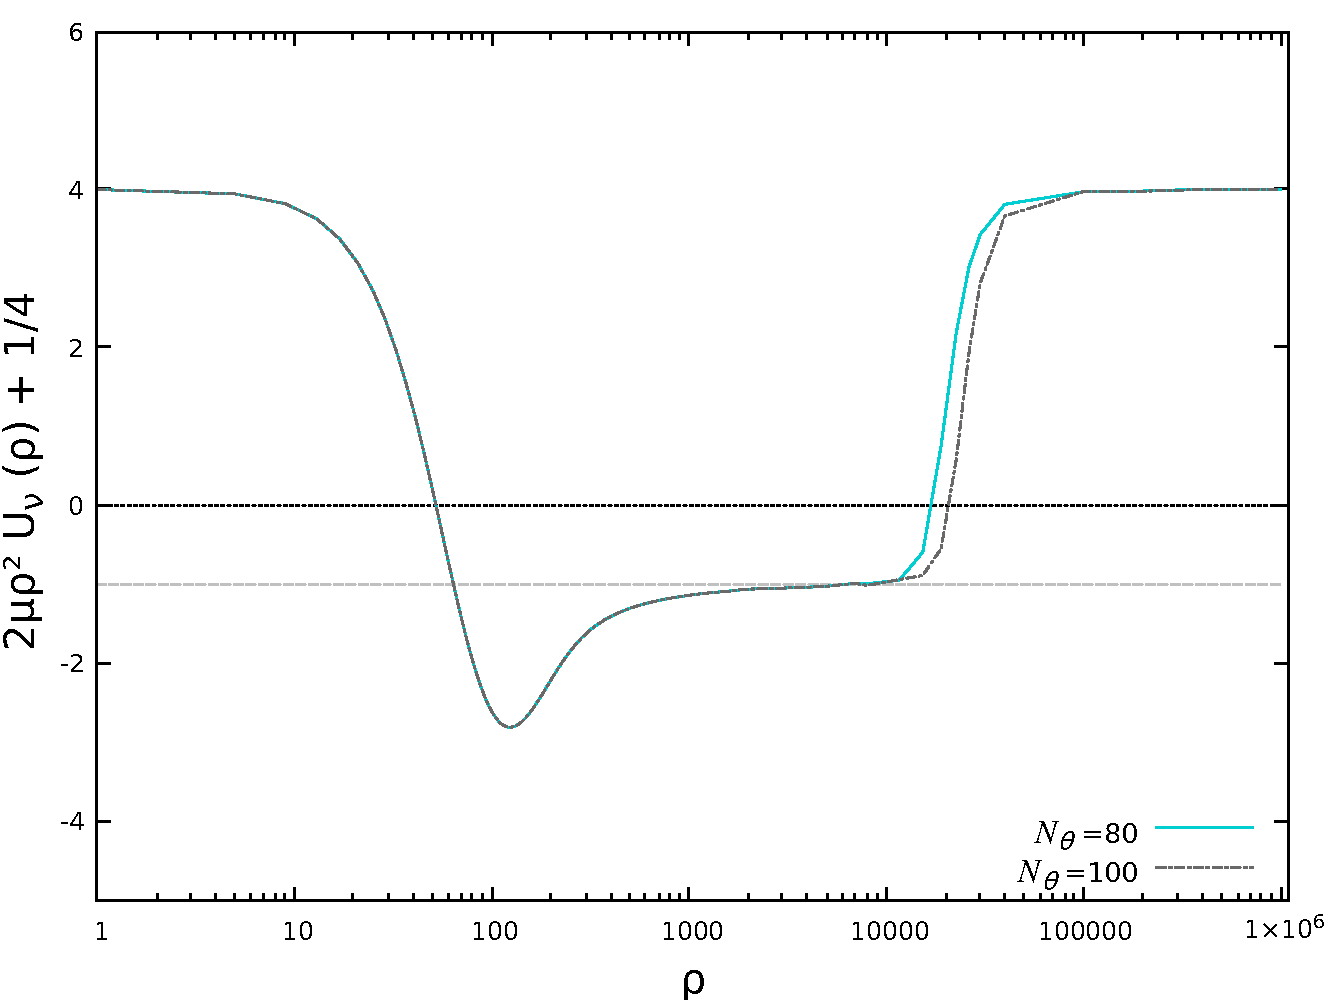
\includegraphics[width=\linewidth]{diffdiff.pdf}
	\caption{Three-body effective potentials for $a=-2702020$ a.u. obtained using $N_{\theta}=N_{\phi}=80$ and $N_{\theta}=N_{\phi}=100$ mesh points, respectively. The potential obtained with $N_{\theta}=0$ converge to $-s_0^2$ for larger $\rho$.}
	\label{fig:res_4}
\end{figure}
In \cref{table:Res_1} we can identify this approximative convergence at $\rho=8000$ a.u. for the potential obtained with $N_{\theta}=100$ mesh points, whereas the potential obtained with $N_{\theta}=80$ mesh points has started to converge to the kinetik energy at this hyperradius.  

\begin{table}[h!]
	\centering
	\begin{tabular}{||c c c||} 
		\hline
		$\rho$ (a.u.) & $N_{\theta}=80$ & $N_{\theta}=100$  \\ [0.5ex] 
		\hline\hline
		8000.0000   & -0.99789324     & -1.01719329  \\ 
		11666.667	 & -0.95232026   & -0.94496812  \\
		15333.333   & -0.59895416  & -0.89254945  \\
		19000.000   & 0.74835108  & -0.55523871   \\
		22666.667   & 2.18632828  & 0.58183597   \\
		26333.333   & 3.01480706  & 1.92849296  \\  
		30000.000   & 3.42706459 & 2.81309001  \\ [1ex] 
		\hline
	\end{tabular}
	\caption{Three-body potential values at different hyperradii for $a = -2702020$ a.u. corrsponding to \cref{fig:res_4}.}
	\label{table:Res_1}
\end{table} 

In \cref{fig:res_4} the potential curves associated with the weakly bound dimer for $a>0$ are plotted as functions of the hyperradius $\rho$, for four different values of $a$. The effective potentials $U_{\nu}$ are expected to converge to the weakly bound channel \eqref{eq:weakdimer}, which energy is approximately given by $-1/ma^2$. This phenomenon should be demonstrated at
large $\rho$ in \cref{fig:res_5} by the $-\rho^2$ divergence of the potential curves. As the magnitude of the scattering length is increased, the effective potential should converge to the Efimov potential (indicated by the horizontal dashed line at $-s_0^2$ in  \cref{fig:res_5}) in the intermediate range $r_0 \ll \rho \ll |a|$. This behaviour can indeed be identified for the potential curve for largest $a$ in \cref{fig:res_5}.

\begin{figure}
	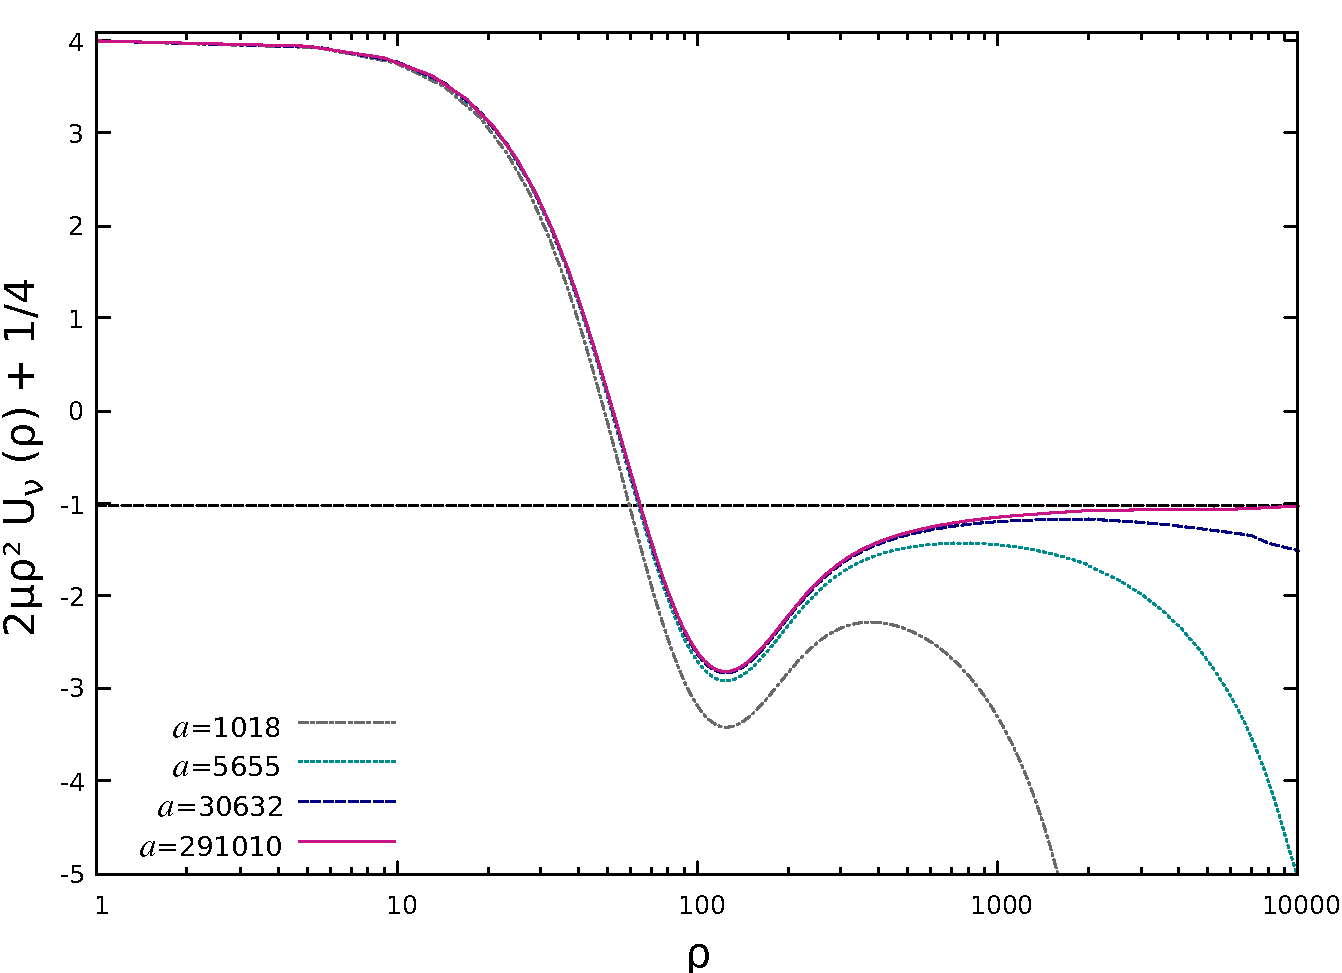
\includegraphics[width=\linewidth]{plotpos.pdf}
	\caption{Three-body effective potentials for $a>0$. The horizontal dashed line is $-s_0^2$.}
	\label{fig:res_5}
\end{figure}

The numerically calculated potentials in the form \eqref{eq:lambda} for two different negative scattering lengths were compared with the analytically derived eigenvalues $\lambda_0(\rho)$ for the hyperangular Faddeev equation \eqref{eq:faddeev_hyperang}. These eigenvalues, obtained at different hyperradii, is an adiabatic potential which correspond to the effective three-body potentials calculated in this work through \eqref{eq:faddeev_effectivepot}. The adiabatic potential $\lambda_0(\rho/\abs{a})$ was determined from the trancendental equation \eqref{eq:transcendental} using \textit{Mathematica}. The analytically derived adibatic potential is plotted together the numerically calculated potentials \eqref{eq:lambda} as functions of $\rho/\abs{a}$ in \cref{fig:res_6,fig:res_7}. Convergence of the potential curves with respect to the B-splines in $\theta$ and $\phi$ was checked by computing them for different numbers of mesh points $N_{\theta}$ and $N_{\theta}$. The convergence of the potential curves for $a=-2385$ a.u. and $a=-8720$ a.u. with an increasing number of mesh points are shown in \cref{fig:res_6,fig:res_7}, respectively. 

\begin{figure}
	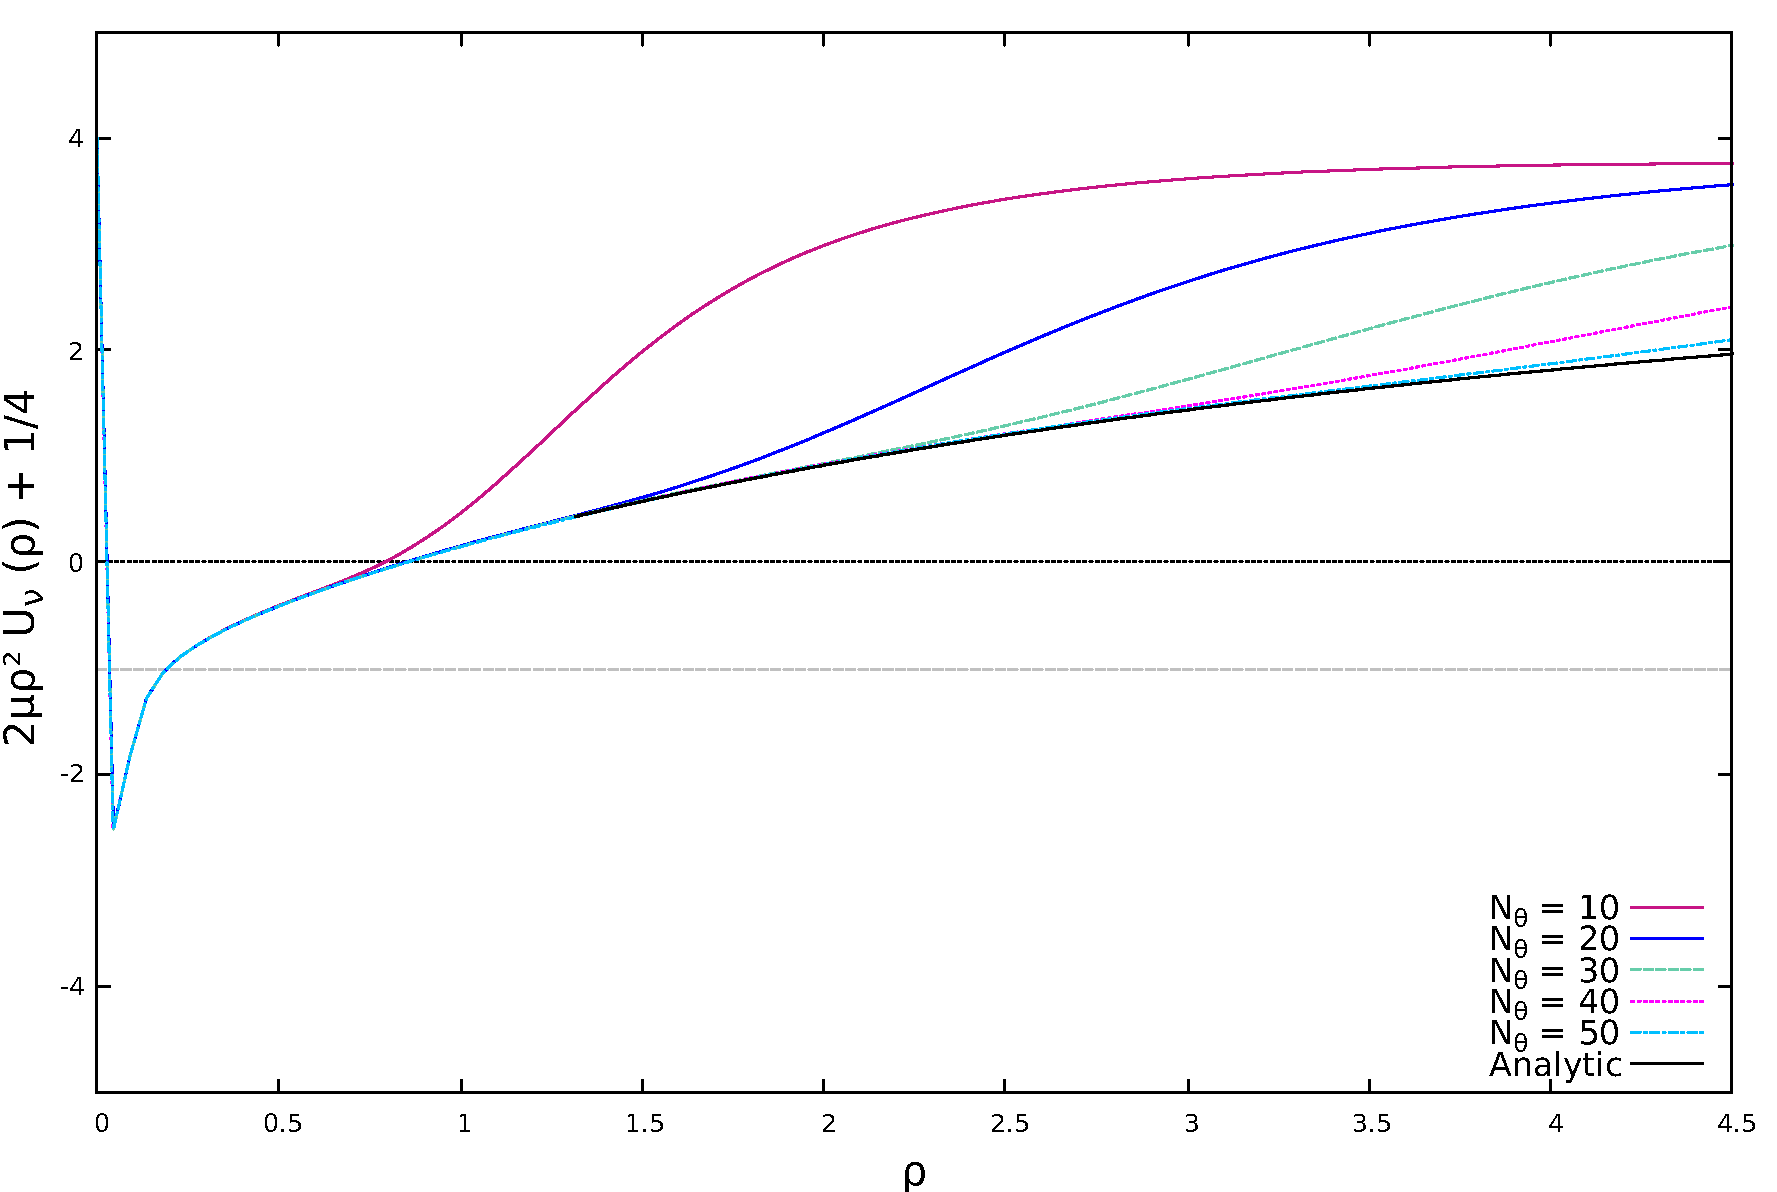
\includegraphics[width=\linewidth]{sn2385.pdf}
	\caption{The convergence towards the analytically derived eigenvalues $\lambda_0$ for $a=-2385$ a.u. is shown for several different numbers of mesh points $N_{\theta}=N_{\phi}$.}
	\label{fig:res_6}
\end{figure}

\begin{figure}
	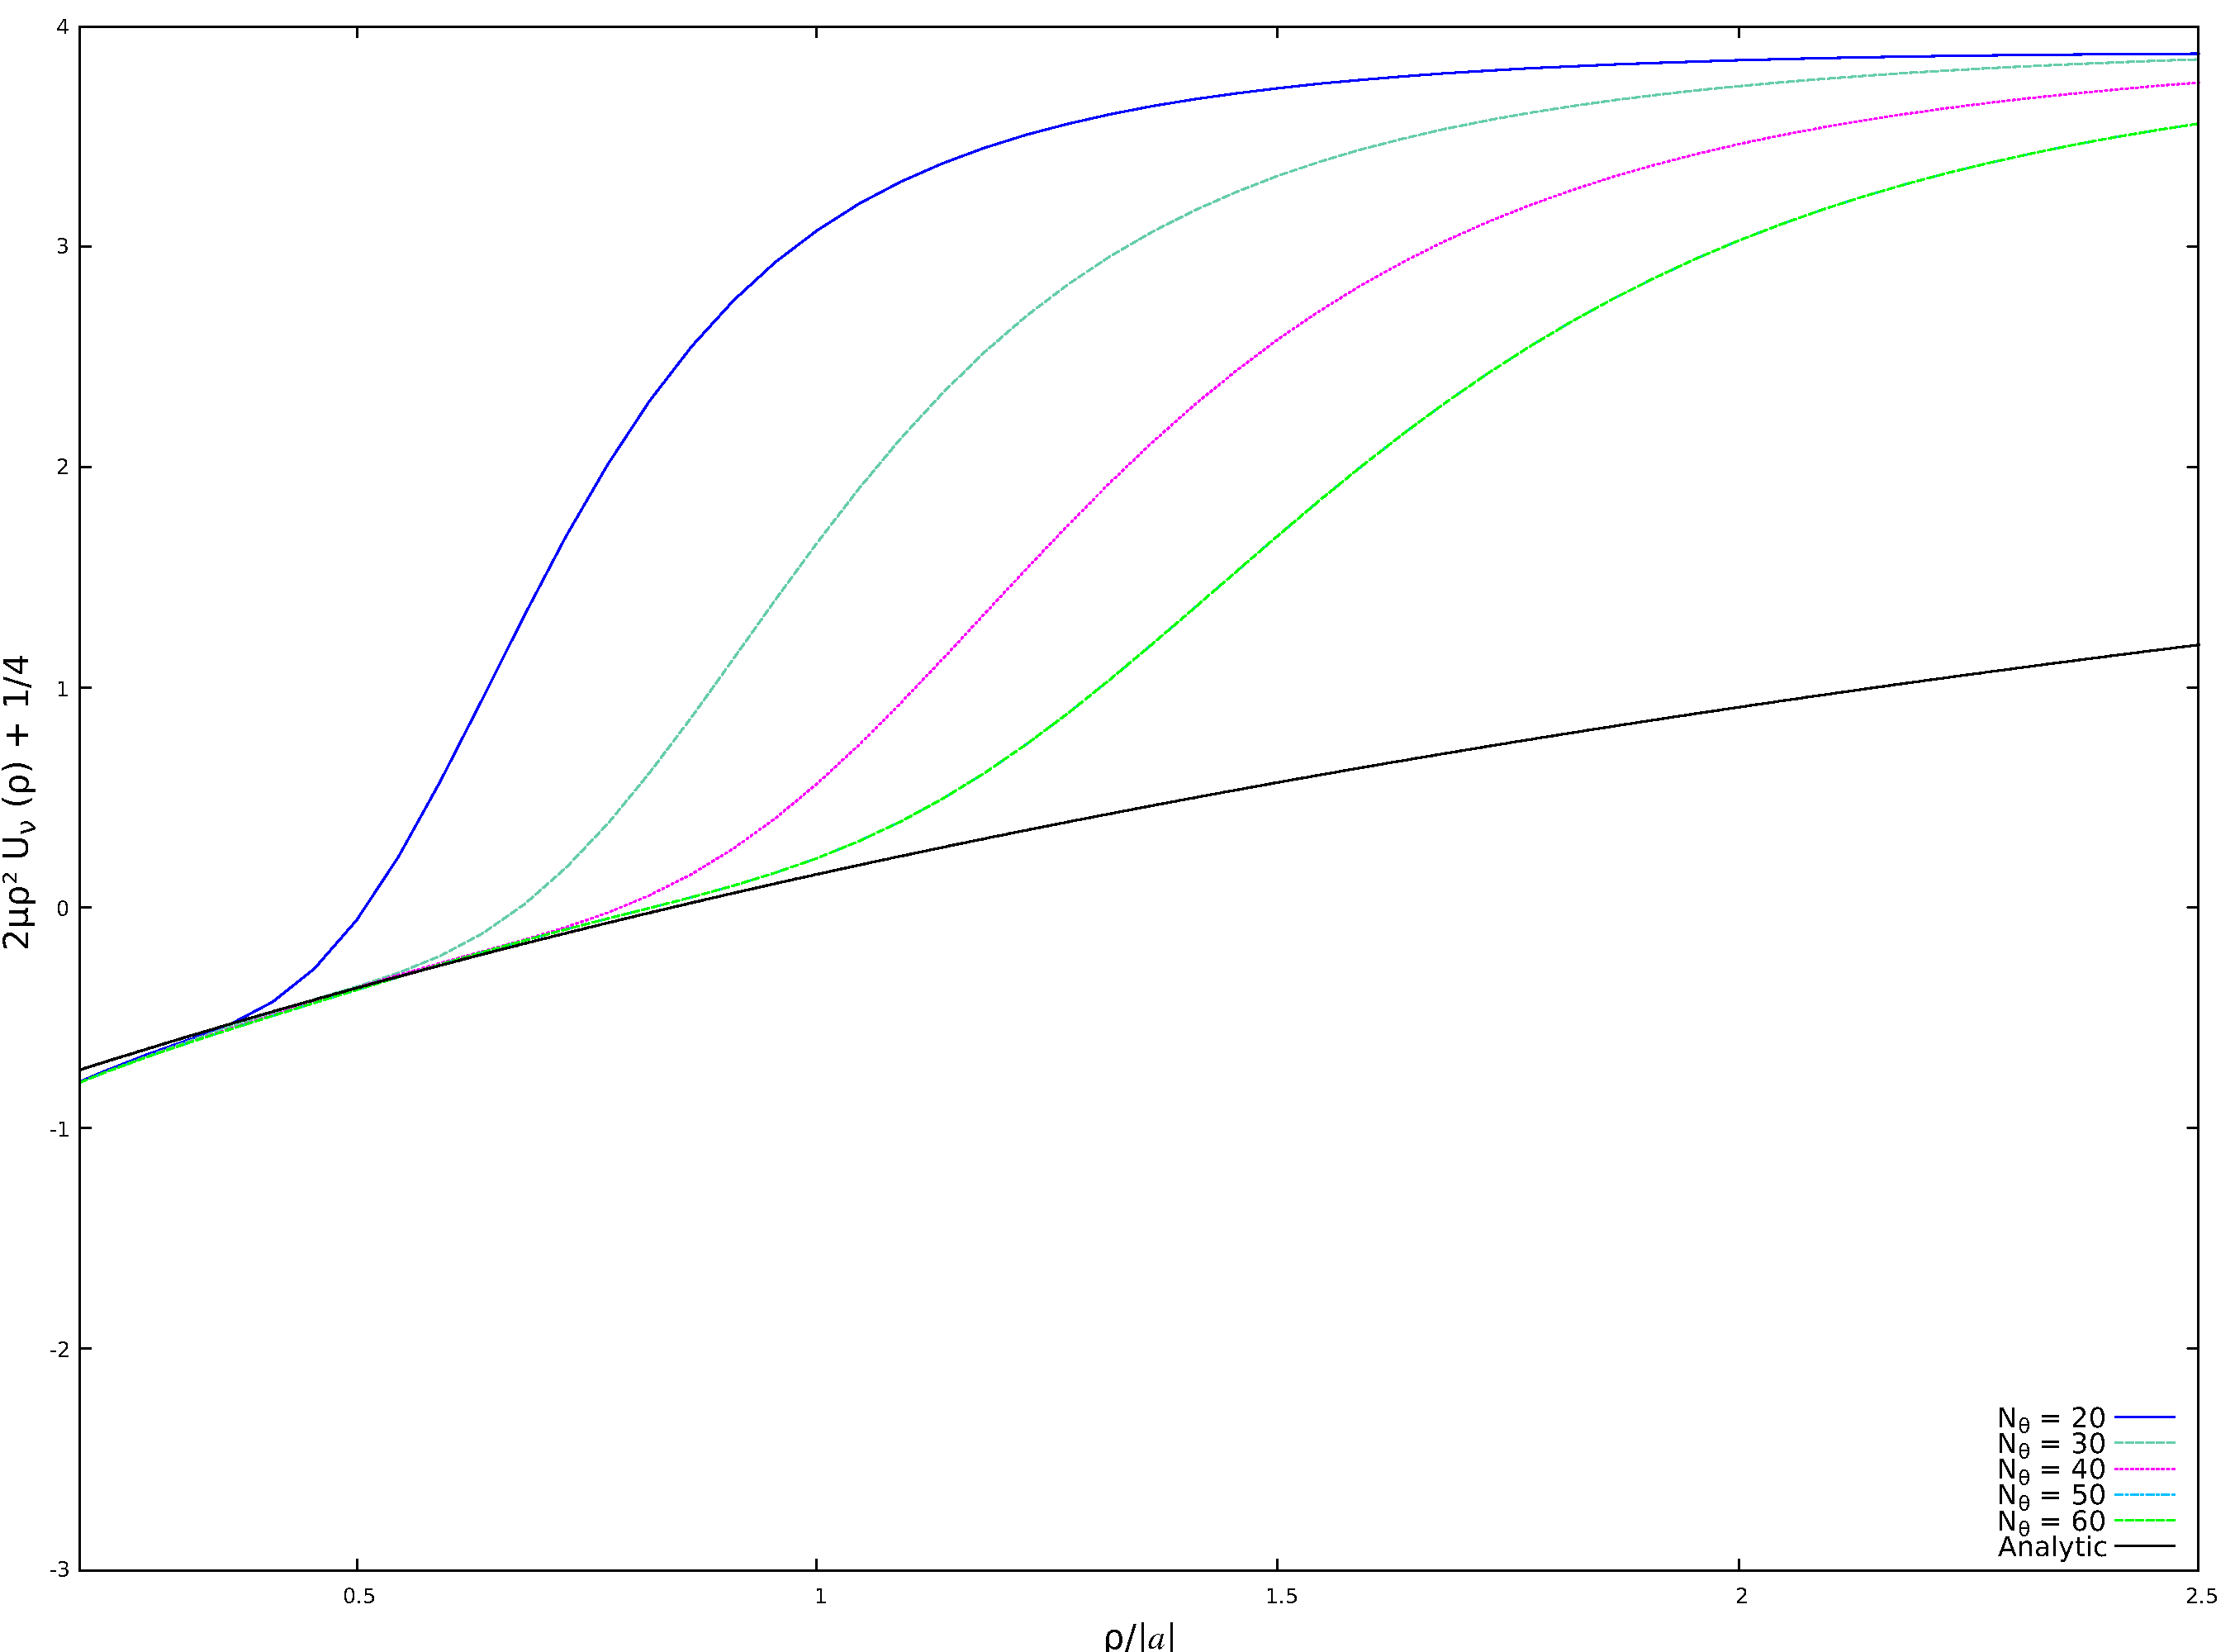
\includegraphics[width=\linewidth]{sn8720.pdf}
	\caption{The convergence towards the analytically derived eigenvalues $\lambda_0$ for $a=-8720$ a.u. is shown for several different numbers of mesh points $N_{\theta}=N_{\phi}$.}
	\label{fig:res_7}
\end{figure}

